
\section{Methodology}
\label{sec:methodology}


\textbf{Roofline Prediction Task.}
The Roofline's Arithmetic Intensity (\rai) is the ratio of floating-point work to DRAM traffic for a kernel invocation.
Rather than ask the models to predict \rai directly, we require them to predict the seven quantities from which \rai is derived:
\begin{itemize}
    \item grid size and block size,
    \item FP16, FP32, and FP64 operation counts, and
    \item DRAM bytes read and DRAM bytes written (on-device).
\end{itemize}
This decomposition makes the task more interpretable and helps in analyzing where a prediction fails.
For example, incorrect launch dimensions imply incorrect thread counts, which in turn propagate to FLOP and memory-traffic errors.

The launch-configuration prediction requires the model to propagate command-line inputs through the host code and recover the first executed kernel launch.
The floating-point operations count prediction then requires reasoning about thread-level work, loop trip counts, control-flow divergence, compiler optimization effects, and operations whose true cost is only partially visible at the source code level.
Finally, the DRAM-traffic prediction requires reasoning about what memory activity actually touches GPU on-board DRAM, rather than merely what appears as source-level loads and stores, including the effect of the GPU's L2 write-back cache on read and write traffic.
After the seven quantities are predicted, we compute \rai separately for FP16, FP32, and FP64 by dividing the predicted FLOP count by the predicted total DRAM bytes moved.
Given a FLOP precision $\texttt{FPXX} \in \{\texttt{FP16}, \texttt{FP32}, \texttt{FP64}\}$, we compute the \rai as follows:
\[
\texttt{\rai}_{\texttt{FPXX}} = \frac{\texttt{FLOP\_Count}_{\texttt{FPXX}}}{\texttt{Bytes\_Read} + \texttt{Bytes\_Written}}.
\]

%\subsection{Benchmark Selection}

%\textbf{Benchmark Selection.} 
%To answer our RQs, we decided to use CUDA and OpenMP codes, as they are two of the most popular GPU programming paradigms \cite{???}.
%Given the diversity of the C++ language and the GPU codes that can be written with it, we turn to the HeCBench suite \cite{HeCBenchMasterZjinlcf} to source a smorgasbord of benchmarks for our experiments.
%We built and profiled 586 HeCBench programs, of which 340 are CUDA, and 246 are OpenMP codes.
%In total, we sampled 1349 GPU kernels: 849 CUDA (built with the \texttt{nvcc} compiler), and 500 OpenMP \texttt{target offload} kernels (built with the \texttt{clang++} compiler).
%We purposely do not balance the CUDA and OpenMP codes in our dataset, to maintain a reflection of reality; these codes range from simulation to math to algorithms codes, so we feel our selection cast a wide-enough net to make conclusions that are broadly applicable to other un-tested CUDA/OpenMP codes.
\textbf{GPU Benchmark Selection.}
%To answer our research questions, we study CUDA and OpenMP GPU programs, two widely-adopted accelerator programming models \cite{kadoshQuantifyingOpenMPStatistical2023}.
%We draw our workloads from the HeCBench suite \cite{HeCBenchMasterZjinlcf, jinBenchmarkSuiteImproving2023}, which contains a broad range of simulation, mathematical, and algorithmic benchmarks.
We study CUDA and OpenMP GPU programs, two widely-adopted accelerator programming models \cite{kadoshQuantifyingOpenMPStatistical2023}, using workloads from the HeCBench suite \cite{HeCBenchMasterZjinlcf, jinBenchmarkSuiteImproving2023}.
From this suite, we build and profile 254 GPU kernels across two runtimes: 155 CUDA and 99 \texttt{target offload} OpenMP kernels.
We preserve the suite's natural CUDA/OpenMP composition rather than artificially balancing the two groups so the study reflects a realistic benchmark mix.
% We intentionally preserve the natural CUDA/OpenMP composition of the suite rather than artificially balancing the two groups, so that the study reflects a realistic mix of available GPU benchmark codes.

%These programs yield 1349 analyzed GPU kernels in the final paper dataset, consisting of 849 CUDA kernels and 500 OpenMP \texttt{target offload} kernels.


\begin{table}[ht]
\centering
\caption{Hardware Specs of Sampled GPUs.}
\label{tab:gpu_specs}
\scriptsize
\setlength{\tabcolsep}{3pt}
\renewcommand{\arraystretch}{1.05}
\resizebox{\columnwidth}{!}{%
\begin{tabular}{@{}p{0.35cm}p{3.25cm}cccc@{}}
\toprule
 &  & \textbf{RTX 3080 (PCIe)} & \textbf{A10 (PCIe)} & \textbf{A100 (SXM4)} & \textbf{H100 (SXM5)} \\
\midrule
 & Base architecture & Ampere (GA102) & Ampere (GA102) & Ampere (GA100) & Hopper (GH100) \\
 & Compute capability & 8.6 & 8.6 & 8.0 & 9.0 \\
 & Base Mem.\ Frequency (MHz) & 9500 & 6251 & 1215 & 1313 \\
 & Base Core Frequency (MHz) & 1440 & 885 & 1095 & 1590 \\
 & SM Count & 68 & 72 & 108 & 132 \\
 & Memory Type & GDDR6X & GDDR6 & HBM2e & HBM3 \\
 & TDP (W) & 320 & 150 & 400 & 700 \\
 & Global Memory Size (GB) & 10 & 24 & 40 & 80 \\
 & Memory Bandwidth (GB/s) & 760 & 600 & 1555 & 3360 \\
 & L2-cache size (MB) & 5 & 6 & 40 & 50 \\
\midrule
\multirow{3}{*}{\rotatebox[origin=c]{90}{\textbf{Per-SM}}}
 & L1-cache size (KB) & 128 & 128 & 192 & 256 \\
 & CUDA cores & 128 & 128 & 64 & 128 \\
 & Shared memory (bytes) & up to 100\,KB & up to 100\,KB & up to 164\,KB & up to 228\,KB \\
\midrule
\addlinespace
%\multirow{3}{*}{\rotatebox[origin=c]{90}{\textbf{Peak Perf.}}}
\multirow{3}{*}{\rotatebox[origin=c]{90}{\textbf{\begin{tabular}{@{}c@{}}Peak Perf.\\(TFLOP/S)\end{tabular}}}}
 & \ \ FP16: Half-Precision & 30.55 & 15.62 & 77.97 & 133.82 \\
 & \ \ FP32: Single-Precision & 30.55 & 15.62 & 19.49 & 66.91 \\
 & \ \ FP64: Double-Precision & 0.477 & 0.244 & 9.75 & 33.45 \\
 & \\
\midrule
\multirow{4}{*}{\rotatebox[origin=c]{90}{\textbf{\begin{tabular}{@{}c@{}}Balance Pt.\\(FLOP/byte)\end{tabular}}}}
 & \\
 & \ \ FP16: Half-Precision & 40.20 & 26.03 & 50.14 & 39.83 \\
 & \ \ FP32: Single-Precision & 40.20 & 26.03 & 12.53 & 19.91 \\
 & \ \ FP64: Double-Precision & 0.63 & 0.41 & 6.27 & 9.96 \\
 & \\
\bottomrule
\end{tabular}%
}
\end{table}


%\textbf{Hardware Selection.}
%We profiled the aforementioned codes on four GPUs: an NVIDIA RTX 3080, A10, A100, and H100.
%\autoref{tab:gpu_specs} provides a high-level comparison of the four GPUs.
%Note how we profile across three different compute-capabilities (\texttt{sm\_80}, \texttt{sm\_86}, \texttt{sm\_90}), with varying memory types/sizes, bandwidths, and peak performances.
%We selected these systems to maximize our work's applicability, as these GPUs were released multiple years apart, and are widely available on consumer/cloud-based platforms \cite{???}.
\textbf{Hardware Selection.}
We profile the benchmark suite on four NVIDIA GPUs: an RTX 3080, A10, A100, and H100.
As summarized in \autoref{tab:gpu_specs}, these devices span three compute capabilities, multiple memory technologies, and substantially different bandwidth and peak-throughput regimes, allowing us to test whether LLM-based arithmetic-intensity prediction generalizes across distinct deployment settings.

%\autoref{tab:gpu_specs} summarizes the hardware characteristics used in the study.
%Together, these devices span three compute capabilities (\texttt{sm\_80}, \texttt{sm\_86}, and \texttt{sm\_90}), multiple memory technologies, and substantially different bandwidth and peak-throughput regimes.
%This diversity is important because our objective is not to characterize a single GPU, but to test whether LLM-based arithmetic-intensity prediction generalizes across distinct architectural generations and deployment settings.



%\textbf{Profiling Design Decisions.}
%W.r.t profiling 1349 GPU kernels, we made some \textbf{\textit{simplifying design decisions}} to avoid exploding our exploration space:
%\begin{enumerate}[label=(\textbf{\arabic*})]
%    \item Profile with the base/default system clock frequencies
%    \item Sample only the first invocation of each kernel 
%    \item Only consider DRAM Arithmetic Intensity (AI)
%\end{enumerate}
%\textit{\textbf{Decision (1)}} was made to minimize the AI prediction space, as peak performance (TFLOP/s) of a system changes w.r.t clock speed, which can change a machine's balance point, altering the definition of when a kernel is considered bandwith/compute bound.
%By keeping the same balance points across profiled codes on a GPU, we can equally compare AI prediction and memory-boundedness classification accuracy.
%\textit{\textbf{Decision (2)}} was made in the interest of not complicating the prediction task.
%The AI of a GPU kernel is profiled for each invocation, this value can change across repeat kernel invocations due to cache-reuse and cross-kernel temporal dependencies. 
%Expecting the LLMs to account for these effects is an additional expectation that complicates the prediction task and subsequent failure mode analysis.
%We stick to asking the LLMs to predict the AI of only the first kernel invocation, as this task proves challenging enough for SoTA LLMs.
%\\\textbf{\textit{Decision (3)}} was made again to shrink the AI prediction space.
%The Roofline model can be expanded so the LLMs predict the AI at each of the caches of a system \cite{ilicCacheawareRooflineModel2014} however, this requires that the LLMs reason about cache reads/writes at each cache level to produce accurate AI predictions.
%When only considering the DRAM Roofline, the LLMs are already expected to reason about DRAM reads/writes that go through an L2 write-back cache; to expect even more reasoning about evictions at the L1 and L2 cache levels only further complicates the task.
%For simplicity of the task space, we keep the above three design decisions, leaving their further analysis as future work.
\textbf{Profiling Design Decisions.}
To keep the prediction task well-defined, we make three simplifying design decisions:
\begin{enumerate}[label=(\textbf{\arabic*})]
    \item profile each GPU at its base/default clock settings,
    \item analyze only the first invocation of each kernel within an executable run, and
    \item restrict the study to DRAM arithmetic intensity.
\end{enumerate}
%Decision (1) keeps each GPU's Roofline balance points fixed throughout the study, which makes cross-kernel and cross-architecture comparisons consistent.
Decision (1) keeps each GPU's Roofline balance points fixed, making cross-kernel and cross-architecture comparisons consistent.
Decision (2) avoids requiring the models to reason about inter-invocation cache reuse and cross-kernel temporal effects, both of which can change inter-invocation traffic.
Decision (3) limits the target to the DRAM-level Roofline rather than a cache-aware variant \cite{ilicCacheawareRooflineModel2014}, allowing us to focus on a single, actionable notion of arithmetic intensity while leaving finer-grained cache-level prediction as a further technical refinement.


\begin{table}[b!]
\centering
\caption{Sampled LLMs sorted by release date with corresponding input/output token costs (as-of March 2026)}
\label{tab:llm_comparison}
\scriptsize
\setlength{\tabcolsep}{3pt}
\renewcommand{\arraystretch}{1.05}
\resizebox{\columnwidth}{!}{%
\begin{tabular}{@{}p{2.2cm}p{1.6cm}p{2.0cm}p{1.5cm}@{}}
\toprule
\textbf{\vfill Model} & \textbf{\vfill Release Date} & \textbf{1e6 Token Cost\newline (in / out)} & \textbf{Max Tokens (in / out)} \\
\midrule
% % GPT-5.1 Codex Mini      & 2025-11-13 & \$0.25 / \$2    & 300K / 100K \\
% % GPT-5.2                 & 2025-12-10 & \$1.75 / \$14   & 272K / 128K \\
% Claude Opus 4.6         & 2026-02-04 & \$5 / \$25      & 872K / 128K \\
% % Claude Sonnet 4.6       & 2026-02-17 & \$3 / \$15      & 936K / 64K \\
% % Gemini 3.1 Pro          & 2026-02-19 & \$2 / \$12      & 983K / 66K \\
% % GPT-5.3 Codex           & 2026-02-24 & \$1.75 / \$14   & 272K / 128K \\
% Gemini 3.1 Flash Lite   & 2026-03-03 & \$0.25 / \$1.50 & 983K / 66K \\
% GPT-5.4                 & 2026-03-05 & \$2.50 / \$15   & 922K / 128K \\
% GPT-5.1 Codex Mini      & 2025-11-13 & \$0.25 / \$2    & 300K / 100K \\
% GPT-5.2                 & 2025-12-10 & \$1.75 / \$14   & 272K / 128K \\
GPT-OSS 120B             & 2025-08-05 & \$0.039 / \$0.19 & 131K / 131K \\
Claude Opus 4.6         & 2026-02-04 & \$5 / \$25      & 872K / 128K \\
% Claude Sonnet 4.6       & 2026-02-17 & \$3 / \$15      & 936K / 64K \\
% Gemini 3.1 Pro          & 2026-02-19 & \$2 / \$12      & 983K / 66K \\
% GPT-5.3 Codex           & 2026-02-24 & \$1.75 / \$14   & 272K / 128K \\
% Nemo 3 Nano 30B     & 2025-12-14 & \$0.05 / \$0.20 & 210K / 52K \\
% Gemini 3 Flash          & 2025-12-17 & \$0.50 / \$3    & 983K / 66K \\
% Gemini 3.1 Flash Lite   & 2026-03-03 & \$0.25 / \$1.50 & 983K / 66K \\
GPT-5.4                 & 2026-03-05 & \$2.50 / \$15   & 922K / 128K \\
% GPT-5.4 Nano            & 2026-03-17 & \$0.20 / \$1.25 & 272K / 128K \\
\bottomrule
\end{tabular}%
}
\end{table}

%\textbf{Dataset Creation.}
%When profiling the 1349 kernels on each GPU, we used NVIDIA's Nsight Compute \texttt{ncu} \cite{4NsightCompute} with \texttt{--set full} flag to gather all the performance counter data for each first invocation.
%We gathered 3 repeat sample invocations of each kernel's executable using the default HeCBench-provided command-line arguments.
%For each kernel, these 3 samples had all their Roofline-related counter metric values averaged to account for any noise during execution.
%
%Once we had the counter data collected, we also scraped all the executables to extract their SASS assembly sections for each kernel via \texttt{cuobjdump}.
%When extracting SASS, we made sure to include the SASS of all the functions called by a kernel (e.g: floating point division slowpaths) to offer a complete picture of the instructions that could be executed.
%
%We next extracted the compile commands used for each executable, as many use pre-processor defines that should be included in LLM prompting to guarantee correct reasoning about source code.
%Given the extracted compile commands, we also scraped the source codes of each executable using the files listed in their compilation commands, making sure to also scrape relevant header files used in compilation.
%This allowed us to include the minimum necessary set of source code files to build/reason about each sampled executable.
%
%\autoref{???} shows an overview of this data collection process.
%Overall, the 1349 kernels profiled across 4 GPUs resulted in a dataset of 5396 datapoints to query, allowing us to study how the LLMs predict the arithmetic intensity of many GPU kernels across 4 different devices.

\begin{figure}[ht]
    \centering
    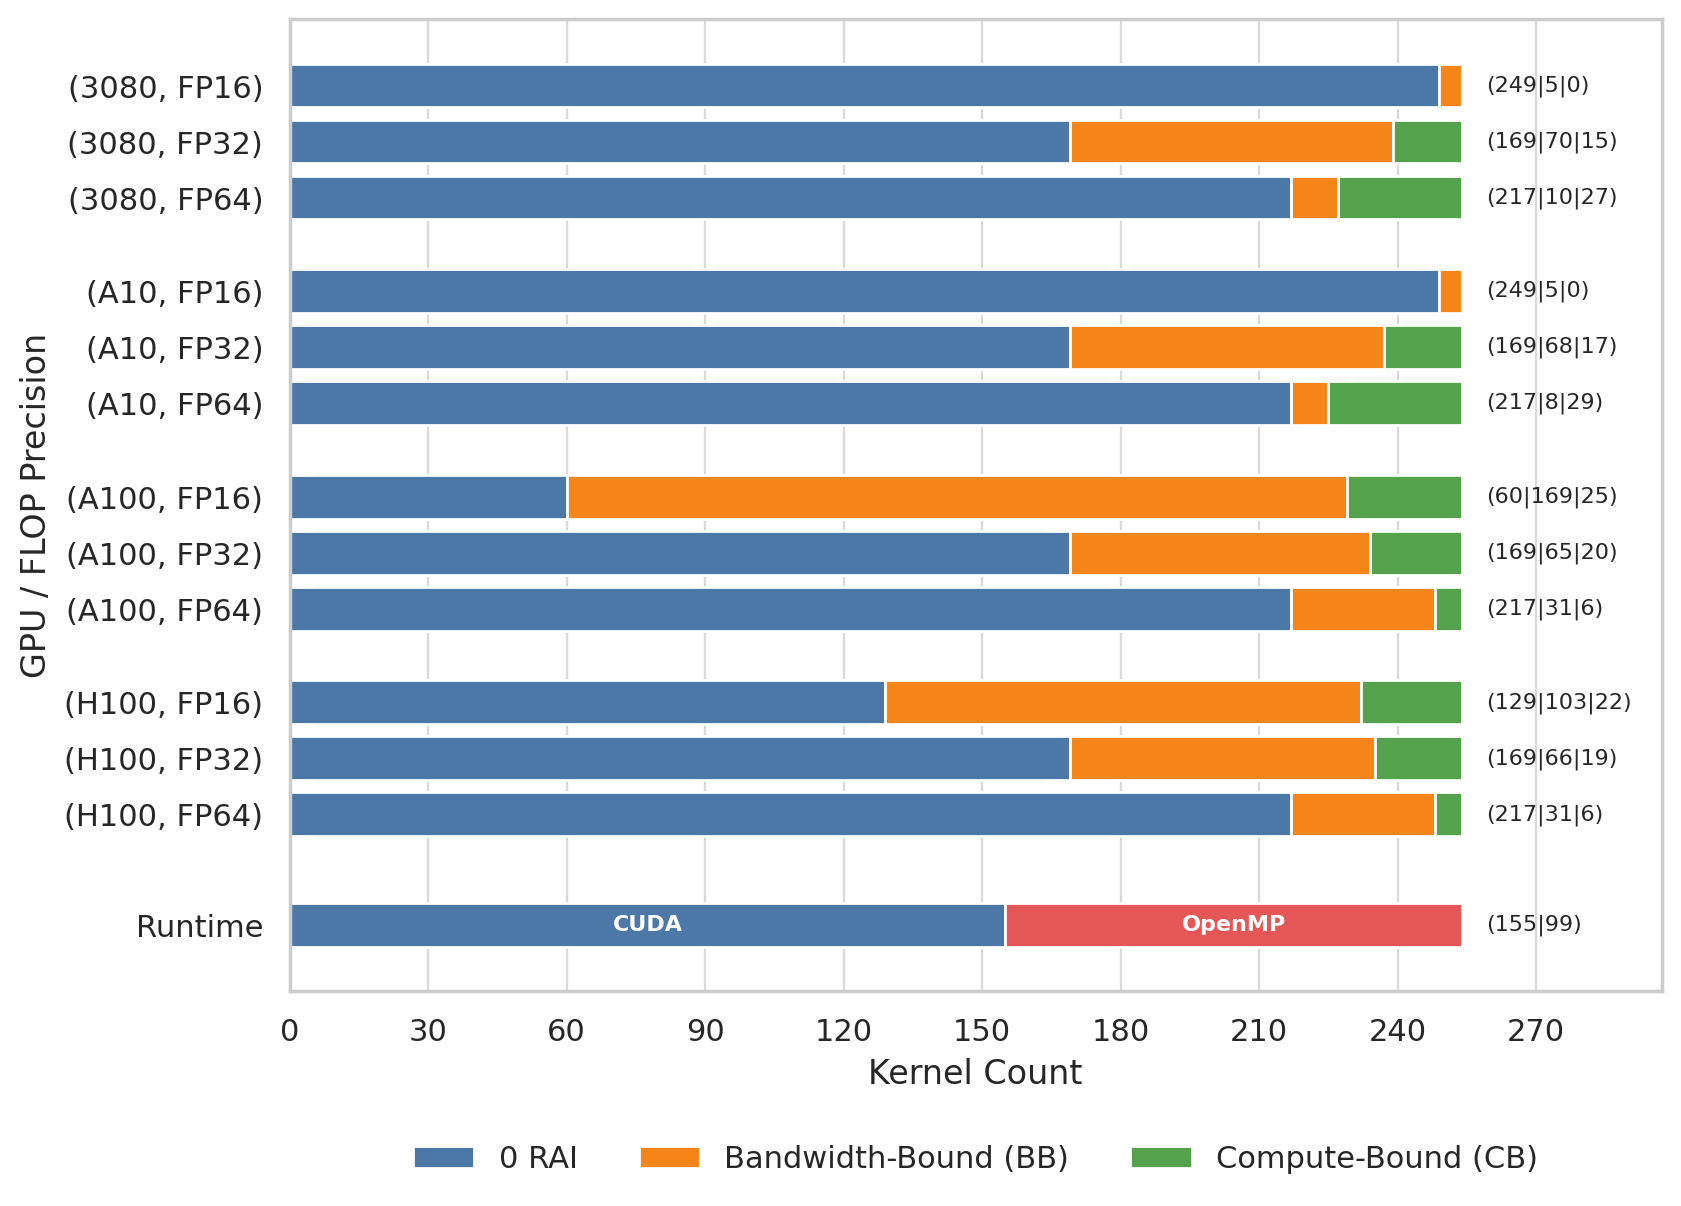
\includegraphics[width=0.95\linewidth]{figures/figure6_expected_rai_distribution_by_gpu_precision.png}
    \caption{Distribution of the profiled arithmetic-intensity classes used later in the paper, split by GPU and floating-point precision.
    Most kernels have zero \rai, while the A100 and H100 contain many more non-zero FP16 cases, motivating evaluation across multiple GPUs rather than a single device.}
    %\caption{Distribution of Bandwidth-Bound and Compute-Bound kernels profiled on each GPU at each FLOP precision.
    %There is a special case of 0 \rai, where a kernel does no FLOP work; this makes up the majority of the kernels at each FLOP precision.
    %There are a total of 254 kernels, whose \rai values vary between GPUs, causing an imbalanced dataset with more CUDA kernels than OpenMP kernels.
    %}
    \label{fig:datasetDistribution}
\end{figure}



\textbf{Dataset Creation.}
For each kernel on each GPU, we collect profiling data with NVIDIA Nsight Compute \texttt{ncu} \cite{4NsightCompute} using the \texttt{--set full} configuration.
We execute each benchmark three times with the default HeCBench command-line arguments and retain profiler statistics for the first invocation of the target kernel in each run.
We then average the Roofline-relevant counters across the three samples to reduce run-to-run noise.

From these profiling runs, we retain the quantities required for arithmetic-intensity analysis: execution time, DRAM bytes read, DRAM bytes written, and FP16/FP32/FP64 operation counts.
For the 254 profiled kernels, \autoref{fig:datasetDistribution} shows the distribution of the Bandwidth-Bound (BB) and Compute-Bound (CB) profiling results for each GPU/FLOP-precision. 
The profiled \rai values are used as ground-truth when querying LLMs to predict \rai.
We note that the majority of the kernels do not perform any FLOPs, resulting in a profiled value of 0 \rai. 
We also note that the A100 and H100 GPUs have many more non-zero FP16-\rai values due to how the compiler injects many more FP16 instructions into their kernel binaries.
These architectural discrepancies highlight the need to study LLM-based \rai predictions across multiple devices.

%We also retain only kernels with valid profiling data on all four GPUs, so that each kernel can be compared consistently across architectures.

In addition to the counter data, we also extract post-compilation artifacts needed for prompting.
We use \texttt{cuobjdump} to collect SASS sections for each target kernel, including relevant helper functions reached by the kernel body (for example, slowpaths used to implement division or transcendental operations).
We also extract the compilation commands for each executable and use them to recover the corresponding source files and relevant headers.
This produces the minimal source-and-artifact bundle needed for the model to reason about a kernel's launch configuration, floating-point work, and DRAM traffic.

\autoref{fig:datasetCreation} shows an overview of this data collection process.
After filtering to kernels with complete four-GPU coverage, the resulting dataset contains 254 kernels evaluated on four devices, yielding 1016 kernel-GPU datapoints to query for each LLM.

\begin{figure}
    \centering
    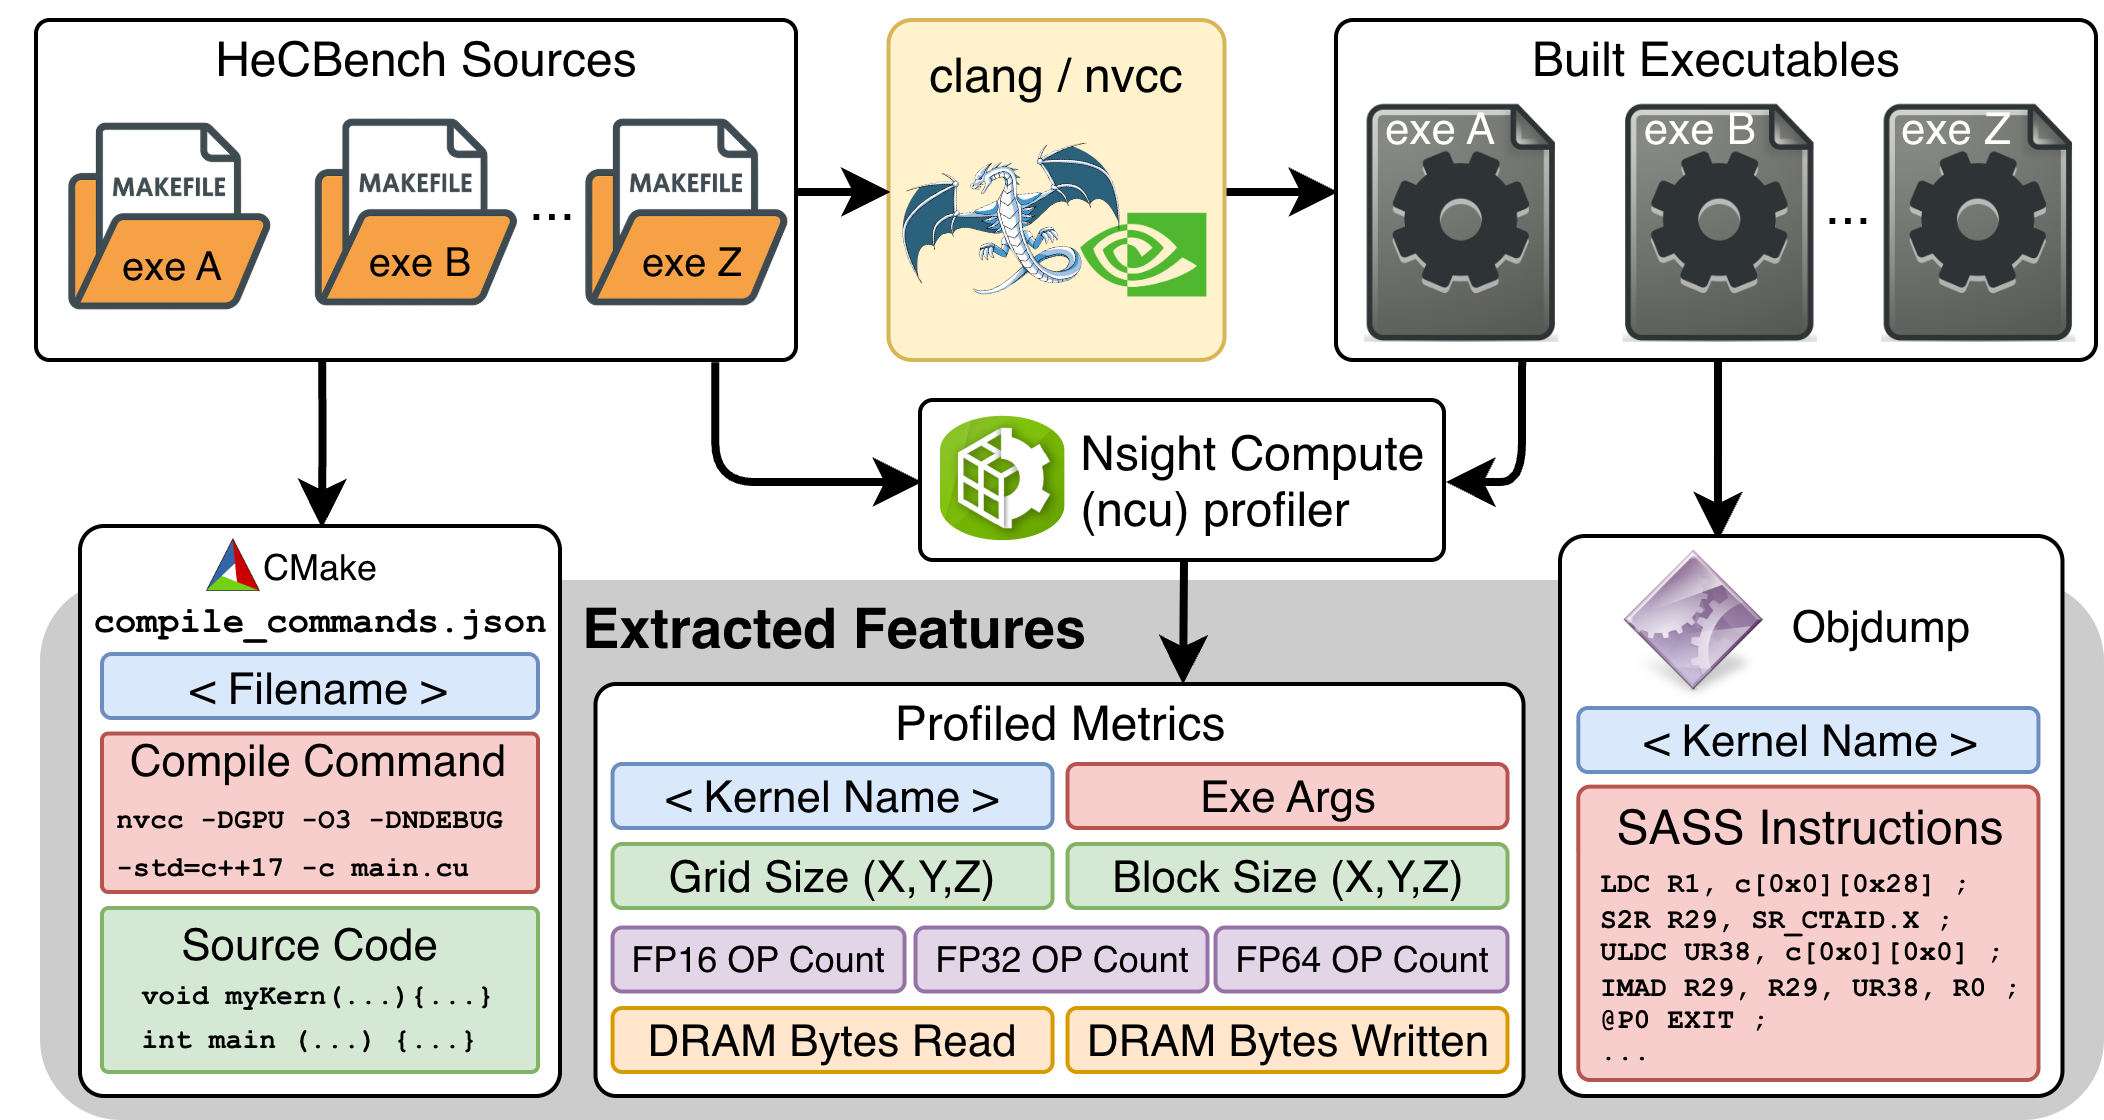
\includegraphics[width=0.95\linewidth]{figures/datasetCreation.png}
    \caption{Dataset-construction pipeline used in this work. 
    For each target kernel, we build the executable, recover the source files, compilation commands, runtime arguments, and SASS, and profile the first invocation to obtain the floating-point and DRAM-traffic ground truth used for prediction.}
    %\caption{The kernel source scraping and profiling approach used in this work.
    %We build CUDA and OpenMP executables from the HeCBench suite, extracting compilation commands, source code, execution metric, and SASS instruction features to use as inputs to the LLMs for static performance prediction.}
    \label{fig:datasetCreation}
\end{figure}


\textbf{Sampled LLMs.}
\autoref{tab:llm_comparison} lists the three models studied in this work: \opus, \gptfivefour, and the cheaper open-source baseline \gptoss.
We focus on the two frontier models to test what off-the-shelf systems can provide without task-specific training, while \gptoss serves as a cost baseline.
This baseline is roughly 100 times cheaper to query than \gptfivefour and \opus.
%\autoref{tab:llm_comparison} lists the LLMs studied in this work.
% Because we have a thousand kernel-GPU combinations, querying the leading LLM models can be quite expensive.
% We limit our comparison to two leading frontier models: Anthropic's \texttt{Opus-4.6} and OpenAI's \texttt{GPT-5.4}.
% Our goal is to evaluate what off-the-shelf models can provide without task-specific training.
% In contrast to the two expensive closed-source models, we studied OpenAI's \texttt{GPT-OSS 120B}, an open-source model released in August of 2025.
% The \gptoss model serves as cost-effective baseline of comparison, as it is 2 orders of magnitude cheaper to query than \gptfivefour and \opus.


\begin{figure}[t!]
    \centering
    
\includegraphics[width=0.9\linewidth]{figures/promptingApproach.png}
    \caption{Per-kernel prompting workflow used for arithmetic-intensity prediction.
    Each query includes the kernel identifier, source code, build context, runtime arguments, and GPU specifications; a second prompt setting additionally includes post-compilation SASS so we can measure how much compiler-realized behavior improves predictions.}
    %\caption{The direct prompting approach studied in this work. 
    %We supply pre-compilation information such as: the target kernel name for prediction, source code including the kernel definition and \texttt{main()} entrypoint of the program, executable arguments, compilation commands, and GPU hardware specification. 
    %We expect the LLM to predict the arithmetic intensity of a program by explicitly counting the number of FLOPs and DRAM Reads/Writes to calculate \rai. 
    %We perform the same queries, but with SASS instructions included to study the influence of post-compilation artifacts on predictions.}
    \label{fig:promptingApproach}
\end{figure}




\textbf{Prompting Approach.}
\autoref{fig:promptingApproach} visualizes our prompting workflow.
Each query supplies the model with the information needed to reason about one target kernel on one target GPU.
The prompt includes: (1) the target kernel name in both mangled and demangled form, (2) the compilation commands, (3) the relevant source files and headers, (4) the executable command-line arguments, (5) the target GPU hardware specifications, and (6) optional kernel-relevant SASS sections.

The kernel identifier is provided in both mangled and demangled forms because low-level artifacts such as SASS refer to mangled symbol names, while source-level reasoning is easier in demangled form.
For OpenMP kernels, we additionally preserve the source-level location information needed to disambiguate the target offload region.
This is important because a single executable may contain multiple kernel definitions, but the model is asked to reason about only one of them.

Compilation commands are included because macros, include paths, and optimization flags can materially affect both the visible source and the compiled behavior.
The associated source files are embedded directly into the prompt and wrapped in XML-style tags so the model can reason over the exact code used to build the executable.
For the source+SASS setting, we additionally provide the kernel's SASS sections, including relevant helper routines, to test whether post-compilation artifacts improve arithmetic-intensity prediction beyond source-only prompting.

The prompt is divided into a system message and a task-specific message.
The system message defines the prediction task and output constraints, while the task-specific message contains the kernel, source, build, runtime, and hardware context.
We enforce structured output through tool calling so that each response returns the seven predicted quantities together with short explanations for each one.
These explanations support both sanity checking and later error analysis.
A full prompting input and output example is available in Appendix \autoref{sec:llmPrompts}.




\textbf{Code Feature Voting.}
In order to understand what causes failures in our \rai predictions, we automatically flagged source code features that could introduce \textit{hidden} FLOPs or DRAM read/write ops post-compilation, causing the LLMs to struggle at deriving proper thread counts, FLOP counts, and memory accesses.
To do this flagging procedure, we fed each source code multiple times into the cheapest LLMs to vote for the presence or absence of these trouble-some code features.
\autoref{fig:llmVotingScheme} visualizes this voting scheme, where we query the \texttt{Nemo 3 Nano}, \texttt{Gemini 3 Flash}, \texttt{Gemini 3.1 Flash Lite}, and \texttt{GPT 5.4 Nano} three times for each source code, for a total of 12 votes to decide each feature. 
We consider a code feature as \textit{present} if more than 50\% of the votes flag it.
The code features were identified by a human expert as contributing to mispredicted \rai. 
Each code feature and it's respective description are detailed in Appendix \autoref{sec:codeFeatureCategoriesAppendix}.

\begin{figure}[t!]
    \centering
    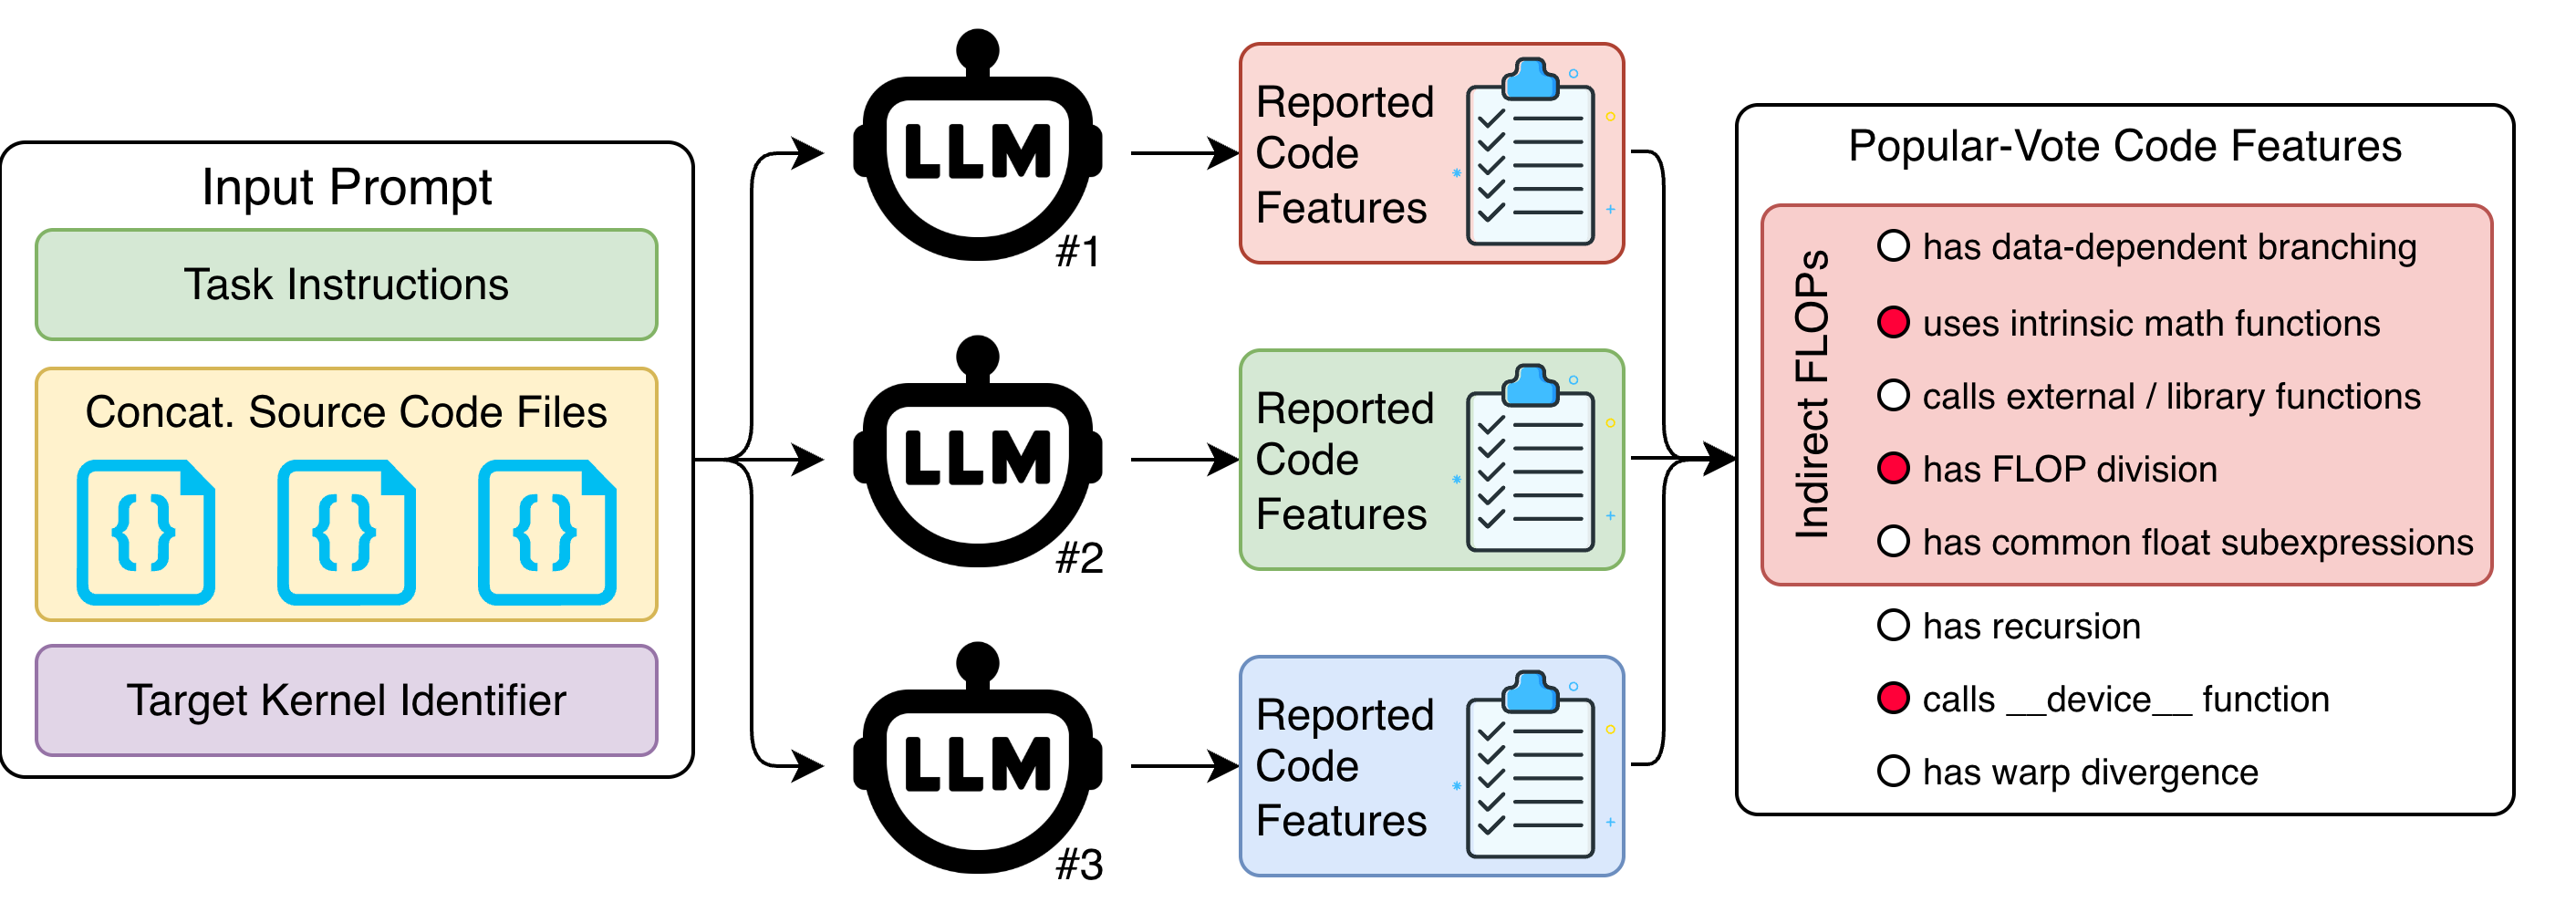
\includegraphics[width=0.98\linewidth]{figures/codeFeatureVoting.drawio.png}
    %\caption{We use an LLM-based voting scheme to categorize the code features present in each kernel. This allows us to classify the CUDA/OpenMP kernels in our dataset according to source-level features that can produce additional \textit{hidden} FLOP operations, often only becoming apparent post-compilation.}
     \caption{Voting ensemble used to label error-prone source features. Four inexpensive LLMs each vote three times per kernel, and a feature is marked present if it receives a majority of the 12 votes.}
    \label{fig:llmVotingScheme}
\end{figure}


\textbf{Evaluation Metrics.}
% Our goal is to evaluate how well current SoTA LLMs predict GPU kernel arithmetic intensity.
% We do so from two complementary perspectives: \textbf{(a)} quantitative \rai error and \textbf{(b)} binary Roofline-class agreement.
% Perspective \textbf{(a)} measures how closely the predicted \rai matches the expected \rai derived from profiling, while perspective \textbf{(b)} asks whether the model correctly identifies a kernel as bandwidth-bound or compute-bound.
% The second perspective is useful because even imperfect \rai estimates may still preserve the optimization-relevant bound classification.
We evaluate the LLMs from two complementary perspectives: \textbf{(a)} quantitative \rai error and \textbf{(b)} binary Roofline-class agreement.
The first measures numerical accuracy against the profiled \rai, while the second asks whether the model preserves the optimization-relevant bound classification.

For perspective \textbf{(a)}, we compute a percent prediction error for each \rai prediction at each FLOP precision.
Given a FLOP precision $\texttt{FPXX} \in \{\texttt{FP16}, \texttt{FP32}, \texttt{FP64}\}$, we compute the percent error as follows:
\[
\text{\% error}_{\texttt{FPXX}} = 100\frac{\text{predicted}_{\texttt{FPXX}} - \text{expected}_{\texttt{FPXX}}}{\text{expected}_{\texttt{FPXX}}}.
\]
% We note that this metric is bounded from the left, as a minimum of -100\% because the smallest prediction value is 0.
% Values less than 0\% are considered under-predictions, while values above 0 are considered over-preditions.
This metric is left-bounded at -100\%, with negative values denoting under-prediction and positive values denoting over-prediction.

For perspective \textbf{(b)}, we compare the predicted and expected binary bound classes using the GPU-specific balance points listed in \autoref{tab:gpu_specs}: a kernel is classified as compute-bound when its \rai exceeds the relevant balance point, and bandwidth-bound otherwise.
Together, these two views measure both numerical error and whether the model preserves the higher-level performance conclusion that would guide optimization effort.



\textbf{Code Feature Error Correlation}
% To measure how strongly each code feature is associated with \rai prediction error, we use \emph{Cliff's Delta}, a nonparametric effect-size measure comparing samples in which a feature is present against samples in which it is absent. 
% For a given feature $f$, let $E_f^{+}$ be the set of absolute \rai prediction errors for samples where $f$ is present, and let $E_f^{-}$ be the set of absolute \rai prediction errors for samples where $f$ is absent. 
To measure how strongly each code feature is associated with \rai prediction error, we use \emph{Cliff's Delta}, a nonparametric effect-size measure comparing feature-present and feature-absent samples.
For a given feature $f$, let $E_f^{+}$ and $E_f^{-}$ denote the sets of absolute \rai prediction errors for samples where $f$ is present and absent, respectively.
Cliff's Delta is defined as

\[
\delta_f
=
\frac{\#(x > y) - \#(x < y)}
{|E_f^{+}| \cdot |E_f^{-}|},
\qquad x \in E_f^{+},\; y \in E_f^{-},
\]

where $\#(x > y)$ counts the number of pairwise comparisons in which the feature-present \textit{absolute} \rai error exceeds the feature-absent \textit{absolute} \rai error, and $\#(x < y)$ counts the number of comparisons in which it is smaller.

The value of $\delta_f$ lies in $[-1,1]$. A value of $\delta_f = 1$ means that every feature-present sample has larger \rai error than every feature-absent sample; $\delta_f = -1$ means the opposite; and $\delta_f = 0$ indicates that neither group consistently dominates the other. 
Thus, positive values indicate that the presence of feature $f$ is associated with higher \rai prediction error, whereas negative values indicate that feature-present kernels tend to have lower \rai error.

We use Cliff's delta because our problem compares a binary predictor (code feature present versus absent) against a continuous error quantity whose distribution is often skewed and may contain outliers. 
Intuitively, if a feature such as ``\textit{Has FLOP Division}'' has $\delta_f = 0.58$, this means that, across all present-versus-absent pairwise comparisons, the FLOP division cases more often have larger \rai error than the non-division cases. 

% In this setting, a rank-based effect size is more informative than a significance test alone, since our goal is to identify which kernel features are most strongly associated with \rai misprediction and in which direction. 















